%%%%%%%%%%%%%%%%%%%%%%%%%%%%%%%%%%%%%%%%%%%%%%%%%%%%%%%%%%%%%%%%%%%%%%
%%  Copyright by Wenliang Du.                                       %%
%%  This work is licensed under the Creative Commons                %%
%%  Attribution-NonCommercial-ShareAlike 4.0 International License. %%
%%  To view a copy of this license, visit                           %%
%%  http://creativecommons.org/licenses/by-nc-sa/4.0/.              %%
%%%%%%%%%%%%%%%%%%%%%%%%%%%%%%%%%%%%%%%%%%%%%%%%%%%%%%%%%%%%%%%%%%%%%%

\newcommand{\commonfolder}{../../common-files}

\documentclass[11pt]{article}

\usepackage[most]{tcolorbox}
\usepackage{times}
\usepackage{epsf}
\usepackage{epsfig}
\usepackage{amsmath, alltt, amssymb, xspace}
\usepackage{wrapfig}
\usepackage{fancyhdr}
\usepackage{url}
\usepackage{verbatim}
\usepackage{fancyvrb}
\usepackage{adjustbox}
\usepackage{listings}
\usepackage{color}
\usepackage{subfigure}
\usepackage{cite}
\usepackage{sidecap}
\usepackage{pifont}
\usepackage{mdframed}
\usepackage{textcomp}
\usepackage{enumitem}
\usepackage{hyperref}


% Horizontal alignment
\topmargin      -0.50in  % distance to headers
\oddsidemargin  0.0in
\evensidemargin 0.0in
\textwidth      6.5in
\textheight     8.9in 

\newcommand{\todo}[1]{
\vspace{0.1in}
\fbox{\parbox{6in}{TODO: #1}}
\vspace{0.1in}
}


\newcommand{\unix}{{\tt Unix}\xspace}
\newcommand{\linux}{{\tt Linux}\xspace}
\newcommand{\minix}{{\tt Minix}\xspace}
\newcommand{\ubuntu}{{\tt Ubuntu}\xspace}
\newcommand{\setuid}{{\tt Set-UID}\xspace}
\newcommand{\openssl} {\texttt{openssl}}


\pagestyle{fancy}
\lhead{\bfseries SEED Labs}
\chead{}
\rhead{\small \thepage}
\lfoot{}
\cfoot{}
\rfoot{}


\definecolor{dkgreen}{rgb}{0,0.6,0}
\definecolor{gray}{rgb}{0.5,0.5,0.5}
\definecolor{mauve}{rgb}{0.58,0,0.82}
\definecolor{lightgray}{gray}{0.90}


\lstset{%
  frame=none,
  language=,
  backgroundcolor=\color{lightgray},
  aboveskip=3mm,
  belowskip=3mm,
  showstringspaces=false,
%  columns=flexible,
  basicstyle={\small\ttfamily},
  numbers=none,
  numberstyle=\tiny\color{gray},
  keywordstyle=\color{blue},
  commentstyle=\color{dkgreen},
  stringstyle=\color{mauve},
  breaklines=true,
  breakatwhitespace=true,
  tabsize=3,
  columns=fullflexible,
  keepspaces=true,
  escapeinside={(*@}{@*)}
}

\newcommand{\newnote}[1]{
\vspace{0.1in}
\noindent
\fbox{\parbox{1.0\textwidth}{\textbf{Note:} #1}}
%\vspace{0.1in}
}


%% Submission
\newcommand{\seedsubmission}{
Debe enviar un informe de laboratorio detallado, con capturas de pantalla, para describir lo que ha hecho y lo que ha observado.
También debe proporcionar una explicación a las observaciones que sean interesantes o sorprendentes.
Enumere también los fragmentos de código más importantes seguidos de una explicación. No recibirán créditos aquellos fragmentos de códigos que no sean explicados.}

%% Book
\newcommand{\seedbook}{\textit{Computer \& Internet Security: A Hands-on Approach}, 2nd
Edition, by Wenliang Du. Para más detalles \url{https://www.handsonsecurity.net}.\xspace}

%% Videos
\newcommand{\seedisvideo}{\textit{Internet Security: A Hands-on Approach},
by Wenliang Du. Para más detalles \url{https://www.handsonsecurity.net/video.html}.\xspace}

\newcommand{\seedcsvideo}{\textit{Computer Security: A Hands-on Approach},
by Wenliang Du. Para más detalles \url{https://www.handsonsecurity.net/video.html}.\xspace}

%% Lab Environment
\newcommand{\seedenvironment}{Este laboratorio ha sido testeado en nuestra imagen pre-compilada de una VM con Ubuntu 16.04, que puede ser descargada del sitio oficial de SEED.\xspace}

\newcommand{\seedenvironmentA}{Este laboratorio ha sido testeado en nuestra imagen pre-compilada de una VM con Ubuntu 16.04, que puede ser descargada del sitio oficial de SEED.\xspace}

\newcommand{\seedenvironmentB}{Este laboratorio ha sido testeado en nuestra imagen pre-compilada de una VM con Ubuntu 20.04, que puede ser descargada del sitio oficial de SEED .\xspace}

\newcommand{\seedenvironmentC}{Este laboratorio ha sido testeado en nuestra imagen pre-compilada de una VM con Ubuntu 20.04, que puede ser descargada del sitio oficial de SEED. Sin embargo, la mayoría de nuestros laboratorios pueden ser realizados en la nube para esto Ud. puede leer nuestra guía que explica como crear una VM de SEED en la nube.\xspace}

\newcommand{\seedenvironmentAB}{
Este laboratorio ha sido testeado en nuestras imagenes pre-compiladas de una VM con Ubuntu 16.04 y otra con Ubuntu 20.04, que pueden ser descargadas del sitio oficial de SEED.\xspace}

\newcommand{\nodependency}{Dado que utilizamos contenedores para configurar el entorno de laboratorio, este laboratorio no depende estrictamente de la VM de SEED. Puede hacer este laboratorio utilizando otras máquinas virtuales, máquinas físicas o máquinas virtuales en la nube.\xspace}

\newcommand{\adddns}{You do need to add the required IP address mapping to
the \texttt{/etc/hosts} file.\xspace}






\newcommand{\seedlabcopyright}[1]{
\vspace{0.1in}
\fbox{\parbox{6in}{\small Copyright \copyright\ {#1}\ \ by Wenliang Du.\\
      Este trabajo se encuentra bajo licencia Creative Commons.
       Attribution-NonCommercial-ShareAlike 4.0 International License.
       Si ud. remezcla, transforma y construye a partir de este material,
       Este aviso de derechos de autor debe dejarse intacto o reproducirse de una manera que sea razonable para el medio en el que se vuelve a publicar el trabajo.
       }}
\vspace{0.1in}
}





\newcommand{\pcap} {\texttt{pcap}\xspace}
\newcommand{\telnet} {\texttt{telnet}\xspace}

\lhead{\bfseries SEED Labs -- Laboratorio de Packet Sniffing y Spoofing}


\begin{document}



\begin{center}
{\LARGE Laboratorio de Packet Sniffing y Spoofing}
\end{center}

\seedlabcopyright{2006 - 2020}


\newcounter{task}
\setcounter{task}{1}
\newcommand{\tasks} {\bf {\noindent (\arabic{task})} \addtocounter{task}{1} \,}

\section{Descripción General}

Los conceptos de Packet sniffing y spoofing, son dos de lo más importantes en el campo de la seguridad de redes; ambos representan las mayores amenazas en las comunicaciones de redes. Poder entender estas amenazas es esencial para comprender las medidas de seguridad en las redes. Existen muchas herramientas para hacer sniffing y spoofing tales como {\tt Wireshark}, {\tt Tcpdump}, {\tt Netwox}, \texttt{Scapy}, etc.
Algunas de ellas son ampliamente usadas por expertos en seguridad como así también por atacantes. Saber usar estas herramientas es algo importante para los estudiantes, pero lo que es más importante para ellos en un curso de seguridad de redes es entender como funcionan esas herramientas, es decir como son implementados el sniffing y spoofing de paquetes en el software.

El objetivo de este laboratorio es doble: El primero es aprender como usar esas herramientas y conocer las tecnologías subyacentes de las mismas.
El segundo será escribir un programa simple para hacer sniffing y spoofing de paquetes y así obtener un conocimiento profundo y detallado de los aspectos técnicos de estos programas.
Este laboratorio cubre los siguientes tópicos:


\begin{itemize}[noitemsep]
\item Como funciona el Packet Sniffing y Spoofing
\item Usando la librería {\tt pcap} y Scapy para hacer Packet sniffing
\item Usando Raw Sockets y Scapy para hacer Packet spoofing 
\item Manipulación de paquetes usando Scapy
\end{itemize}



\paragraph{Lecturas y Videos.}
Para una cobertura más detallada sobre Sniffing y Spoofing puede consultar


\begin{itemize}
\item Capítulo 15 del Libro de SEED, \seedbook
\item Sección 2 del curso de SEED en Udemy, \seedisvideo
\end{itemize}



\paragraph{Entorno de Laboratorio.} \seedenvironmentC



\paragraph{Nota para los intructores.}
En este Laboratorio existen dos Sets de Tareas. El primer set se centra en el uso de herramientas para hacer packet sniffing y spoofing. Esto sólo requiere un conocimiento mínimo en Python; los estudiantes no necesitan tener un background previo de programación en Python.
El segundo set de tareas está pensado para estudiantes de Ciencias de la Computación/Ingeniería. 
Los estudiantes deberán escribir sus propios programas desde cero usando el lenguaje C para llevar a cabo el sniffing y el spoofing de paquetes. De esta forma podrán entender en mayor profundidad como es el funcionamiento de un sniffer y de un spoofer. Para abordar esta tarea, es necesario que los estudiantes tenga un sólido conocimiento en el lenguaje de programación C.
Ambos Sets de Tareas son independientes; los instructores en base al background de programación que tengan sus estudiantes pueden elegir asignar un sólo Set o ambos.



% *******************************************
% SECTION
% ******************************************* 
\section{Configuración del entorno usando Contenedores} 

En este laboratorio, usaremos dos máquinas conectadas a la misma LAN. Podemos usar dós Máquinas Virtuales o dos Contenedores. 
La Figura \ref{fig:labsetup} describe la configuración del entorno de laboratorio utilizando Contenedores.
Realizaremos todos los ataques desde el Contenedor del atacante, mientras que el otro contenedor será la máquina del usuario.

\begin{figure}[htb]
\begin{center}
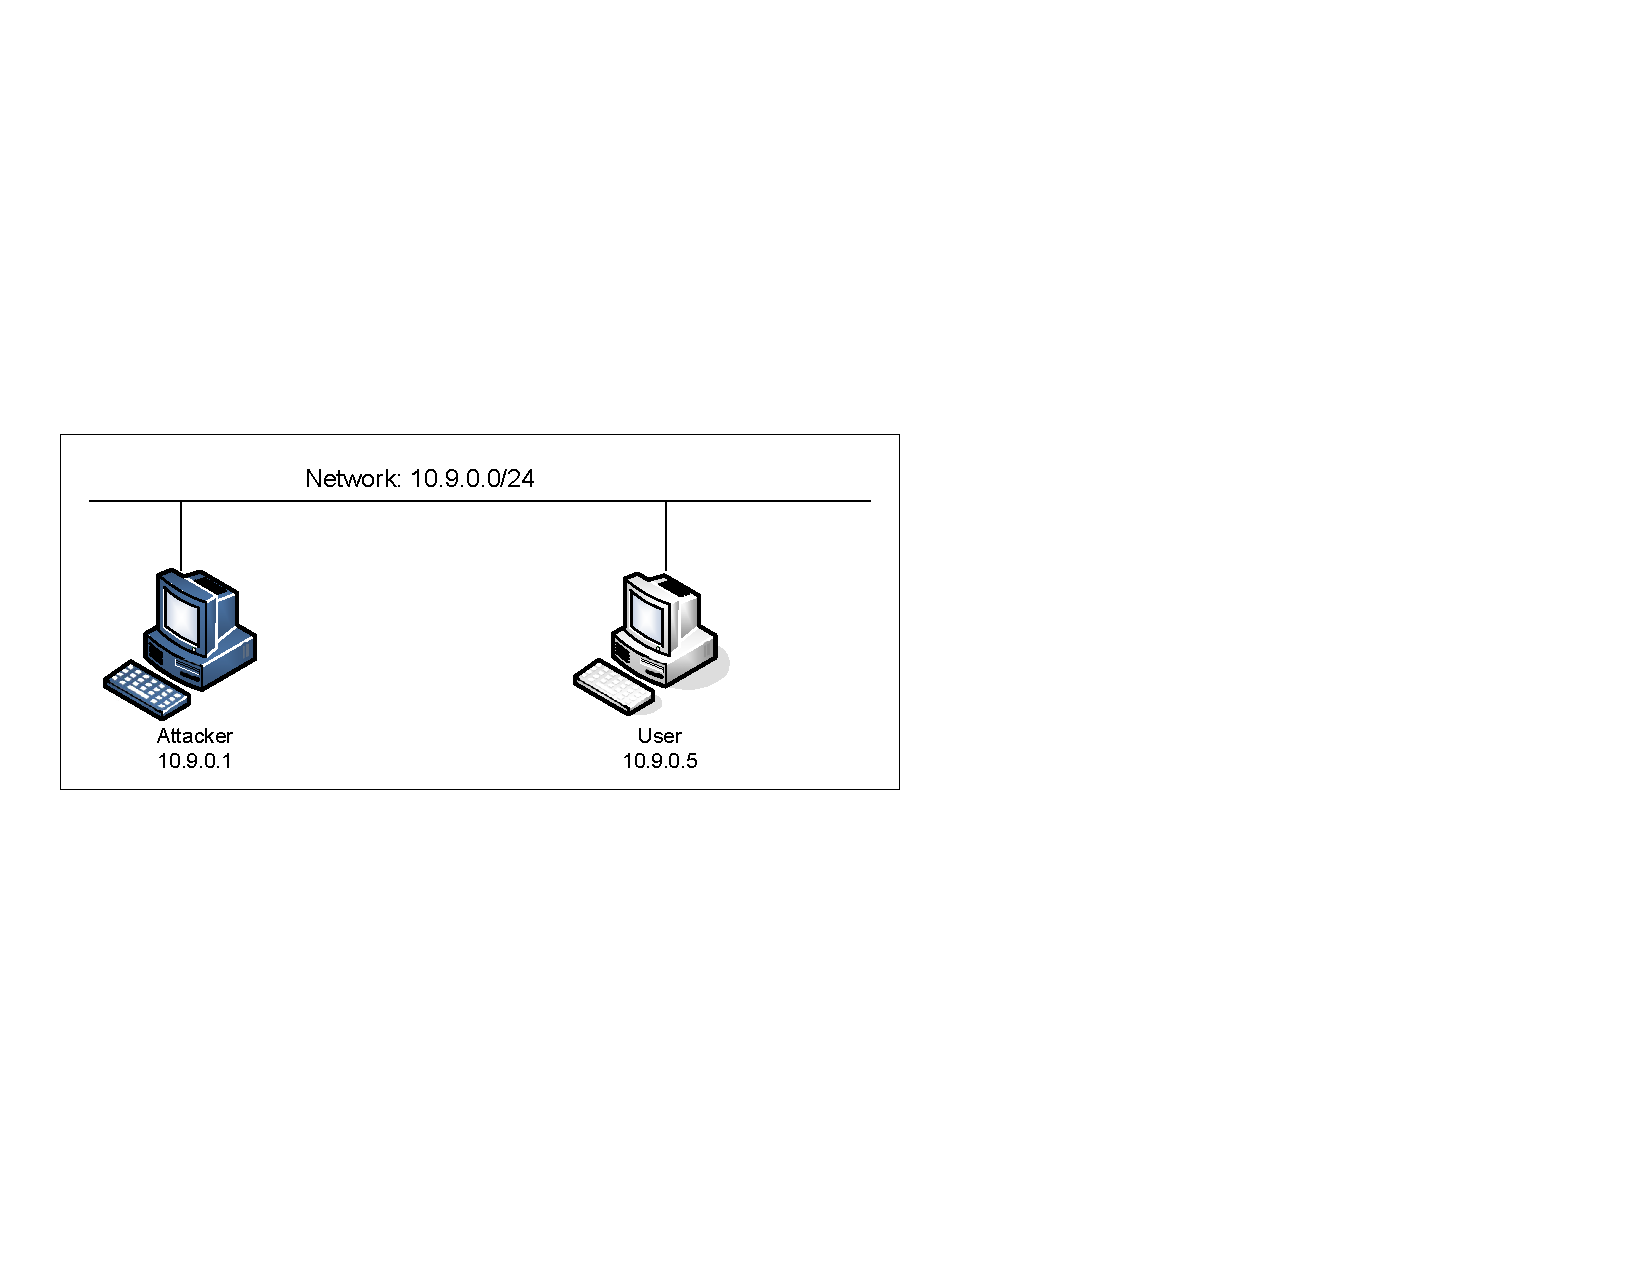
\includegraphics[width=0.8\textwidth]{\commonfolder/Figs/OneLan_onehost.pdf}
\end{center}
\caption{Configuración del entorno}
\label{fig:labsetup}
\end{figure}
 

%\begin{lstlisting}[backgroundcolor=]
%                +--------------+      +--------------+
%                |  (attacker)  |      |    (user)    |
%                |   10.9.0.1   |      |   10.9.0.5   |
%                +-----+--------+      +------+-------+
%                      | br-<id>              | eth0
%         10.9.0.0/24  |                      |
%         -------------+----------------------+------------
%
%\end{lstlisting}
 


% -------------------------------------------
% SUBSECTION
% -------------------------------------------
\subsection{Setup del Contenedor y sus Comandos} 

%%%%%%%%%%%%%%%%%%%%%%%%%%%%%%%%%%%%%%%%%%%%
Para empezar a preparar el contenedor, deberá descargarse el archivo \texttt{Labsetup.zip} ubicado en el laboratorio correspondiente dentro del sitio web oficial y copiarlo dentro de la Máquina Virtual prevista por SEED. Una vez descargado deberá descomprimirlo y entrar dentro del directorio \texttt{Labsetup} donde encontrará el archivo \texttt{docker-compose.yml} que servirá para setear el entorno de laboratorio. Para una información más detallada sobre el archivo \texttt{Dockerfile} y otros archivos relacionados, puede encontrarla dentro del Manual de Usuario del laboratorio en uso, en el sitio web oficial de SEED.

Si esta es su primera experiencia haciendo el setup del laboratorio usando contenedores es recomendable que lea el manual anteriormente mencionado.

A continuación, se muestran los comandos más usados en Docker y Compose.
Debido a que estos comandos serán usados con mucha frecuencia, hemos creados un conjunto de alias para los mismos, ubicados en del archivo \texttt{.bashrc} dentro de la Máquina Virtual provista por SEED (Ubuntu 20.04)

\begin{lstlisting}
$ docker-compose build  # Build the container image
$ docker-compose up     # Start the container
$ docker-compose down   # Shut down the container

// Aliases for the Compose commands above
$ dcbuild       # Alias for: docker-compose build
$ dcup          # Alias for: docker-compose up
$ dcdown        # Alias for: docker-compose down
\end{lstlisting}


Dado que todos los contenedores estarán corriendo en un segundo plano. Necesitamos correr comandos para interactuar con los mismos, una de las operaciones fundamentales es obtener una shell en el contenedor. 
Para este propósito usaremos \texttt{"docker ps"} para encontrar el ID del contenedor deseado y ingresaremos \texttt{"docker exec"} para correr una shell en ese contenedor.
Hemos creado un alias para ello dentro del archivo \texttt{.bashrc}

\begin{lstlisting}
$ dockps        // Alias for: docker ps --format "{{.ID}}  {{.Names}}" 
$ docksh <id>   // Alias for: docker exec -it <id> /bin/bash

// The following example shows how to get a shell inside hostC
$ dockps
b1004832e275  hostA-10.9.0.5
0af4ea7a3e2e  hostB-10.9.0.6
9652715c8e0a  hostC-10.9.0.7

$ docksh 96
root@9652715c8e0a:/#  

// Note: If a docker command requires a container ID, you do not need to 
//       type the entire ID string. Typing the first few characters will 
//       be sufficient, as long as they are unique among all the containers. 
\end{lstlisting}

En caso de problemas configurando el entorno, por favor consulte la sección ``Common Problems'' en el manual ofrecido por SEED. 


%%%%%%%%%%%%%%%%%%%%%%%%%%%%%%%%%%%%%%%%%%%%


% -------------------------------------------
% SUBSECTION
% -------------------------------------------
\subsection{El Contenedor del Atacante}

Para este laboratorio, podemos usar la Máquina Virtual o el Contenedor como la máquina del Atacante. Si hecha un vistazo al archivo de Docker Compose, verá que el contenedor del Atacante está configurado de manera diferente del resto de los contenedores. 
Estas son las diferencias:


\begin{itemize}
\item \textit{Directorio Compartido.} Cuando usemos el contenedor del atacante para lanzar los ataques, necesitamos poner el código de ataque dentro del contenedor.

%%%%%%%%%%%%%%%%%%%%%%%%%%%%%%%%%%%%%%%%%%%%%%%
Code editing is more convenient inside the VM than in containers, 
because we can use our favorite editors.
In order for the VM and container to share files, 
we have created a shared folder between the VM and the container
using the Docker \texttt{volumes}.
If you look at the Docker Compose file, you will find out that
we have added the following entry to some of the containers.
It indicates mounting the \texttt{./volumes} folder on the host
machine (i.e., the VM) to the \texttt{/volumes} folder inside the container.
We will write our code in the \texttt{./volumes} folder (on the VM), so they
can be used inside the containers.

\begin{lstlisting}
volumes:
       - ./volumes:/volumes
\end{lstlisting}


%%%%%%%%%%%%%%%%%%%%%%%%%%%%%%%%%%%%%%%%%%%%%%%


\item \textit{Modo Host.}
%%%%%%%%%%%%%%%%%%%%%%%%%%%%%%%%%%%%%%%%%%%%%%%
In this lab, the attacker needs to be able to sniff packets,
but running sniffer programs inside a container has problems, because
a container is effectively attached to a virtual switch, 
so it can only see its own traffic, and it is never going to see 
the packets among other containers. To solve this problem,
we use the \texttt{host} mode for the attacker container. This
allows the attacker container to see all the traffics. The following
entry used on the attacker container:

\begin{lstlisting}
network_mode: host
\end{lstlisting}

When a container is in the \texttt{host} mode,  it sees
all the host's network interfaces, and it even has the same
IP addresses as the host. Basically, it is put in the
same network namespace as the host VM. However, the container
is still a separate machine, because its other namespaces are
still different from the host.


%%%%%%%%%%%%%%%%%%%%%%%%%%%%%%%%%%%%%%%%%%%%%%%
\end{itemize}


\paragraph{Obteniendo el nombre de la interfaz de red.}
%%%%%%%%%%%%%%%%%%%%%%%%%%%%%%%%%%%%%%%%%%%%%%%
When we use the provided Compose file to create
containers for this lab, a new network is created
to connect the VM and the containers. The
IP prefix for this network is \texttt{10.9.0.0/24},
which is specified in the \texttt{docker-compose.yml}
file. The IP address assigned to our VM is
\texttt{10.9.0.1}. We need to find the name of
the corresponding network interface on our VM, because we
need to use it in our programs.
The interface name is the concatenation of \texttt{br-}
and the ID of the network created by Docker.
When we use \texttt{ifconfig} to list network interfaces,
we will see quite a few. Look for the IP address
\texttt{10.9.0.1}.


\begin{lstlisting}
$ ifconfig
(*@\textbf{br-c93733e9f913}@*): flags=4163<UP,BROADCAST,RUNNING,MULTICAST>  mtu 1500
        inet (*@\textbf{10.9.0.1}@*)  netmask 255.255.255.0  broadcast 10.9.0.255
        ...
\end{lstlisting}


Another way to get the interface name is to use the \texttt{"docker network"} command to
find out the network ID ourselves (the name of the network is \texttt{seed-net}:

\begin{lstlisting}
$ docker network ls
NETWORK ID          NAME                DRIVER              SCOPE
a82477ae4e6b        bridge              bridge              local
e99b370eb525        host                host                local
df62c6635eae        none                null                local
(*@\textbf{c93733e9f913}@*)        seed-net            bridge              local
\end{lstlisting}



%%%%%%%%%%%%%%%%%%%%%%%%%%%%%%%%%%%%%%%%%%%%%%%



% *******************************************
% SECTION
% ******************************************* 
\section{Set 1 de Tareas: Usando Scapy para el Sniffing and Spoofing de Paquetes}

Se pueden utilizar muchas herramientas para hacer sniffing y spoofing pero la mayoría ofrece funciones limitadas. Scapy es diferente: puede ser usada no sólo como una herramienta sino también como módulo para construir herramientas de sniffing y spoofing es decir podemos integrar funcionalidades de Scapy en nuestros propios programas. En este Set de Tareas usaremos Scapy.

Para usar Scapy, podemos escribir un programa en Python y ejecutarlo usando este interpréte. Vea el siguiente ejemplo. Debemos correr este programa de Python usando privilegios de root, dado que son necesarios para realizar operaciones de spoofing sobre paquetes.
Al comienzo del programa (Línea \ding{192}), importamos todos los módulos de Scapy.

\begin{lstlisting}
# view mycode.py
#!/usr/bin/env python3

from scapy.all import *    (*@\ding{192}@*)

a = IP()
a.show()

# python3 mycode.py
###[ IP ]###
  version   = 4
  ihl       = None
  ...


// Make mycode.py executable (another way to run python programs)
# chmod a+x mycode.py
# mycode.py 
\end{lstlisting}

Podemos utilizar el modo interactivo de Python y correr nuestro programa línea a línea. Esto puede ser más conveniente si necesitamos cambiar de forma frecuente nuestro código en un experimento.


\begin{lstlisting}
# python3
>>> from scapy.all import *
>>> a = IP()
>>> a.show()
###[ IP ]###
  version   = 4
  ihl       = None
  ...
\end{lstlisting}
 

% -------------------------------------------
% SUBSECTION
% ------------------------------------------- 
\subsection{Tarea 1.1: Sniffing de Paquetes}  

Una de las herramientas más populares para hacer sniffing es Wireshark, aprender a usar esta herramienta es sencillo y la usaremos durante todo el laboratorio. Sin embargo es difícil usar Wireshark para integrarlo a nuestras aplicaciones y crear módulos con diversas funcionalidades. Para este propósito usaremos Scapy. El objetivo de esta Tarea es aprender a usar Scapy para hacer sniffing de paquetes a través de programas de Python.
A continuación se da un ejemplo:


\begin{lstlisting}
#!/usr/bin/env python3
from scapy.all import *

def print_pkt(pkt):
  pkt.show()

pkt = sniff(iface='br-c93733e9f913', filter='icmp', prn=print_pkt)
\end{lstlisting}

El código mostrado anteriormente, hará sniffing de todos los paquetes en la interfaz \texttt{br-c93733e9f913}. Por favor lea las instrucciones en la sección del Setup del Contenedor para saber como obtener esta interfaz.
Si queremos hacer sniffing en más de una interfaz, podemos usar una lista de python y asignarlas a una variable, en este caso la llamaremos \texttt{iface}.
A continuación se da un ejemplo:

\begin{lstlisting}
iface=['br-c93733e9f913', 'enp0s3']
\end{lstlisting}
 


\paragraph{Tarea 1.1A.} En el programa anterior, por cada paquete capturado, la función \texttt{print\_pkt()} será invocada como un callback; esta función mostrará información detallada del paquete. Ejecute el programa con privilegios de root y demuestre como captura los paquetes. Después de eso corra el programa sin privilegios de root; Describa y explique sus observaciones.
 
\begin{lstlisting}
// Make the program executable 
# chmod a+x sniffer.py

// Run the program with the root privilege
# sniffer.py

// Switch to the "seed" account, and
// run the program without the root privilege
# su seed
$ sniffer.py
\end{lstlisting}


\paragraph{Tarea 1.1B.} Generalmente, cuando hacemos sniffing de paquetes, estamos interesados en ciertos tipos de paquetes y no en todos. Para ello usaremos filtros al hacer el sniffing, estos filtros provistos por Scapy usan la sintáxis BPF (Berkeley Packet Filter); Puede encontrar más información sobre BPF en el manual oficial. Por favor  use los siguientes filtros mencionados a continuación y corra el programa nuevamente (Cada filtro debe ser seteado en forma separada):

\begin{itemize} 
 \item Capturar solamente paquetes ICMP.
 \item Capturar cualquier paquete TCP que provenga de una IP y cuyo puerto destino sea el puerto 23.
  \item Capturar paquetes que vienen o se dirigen hacia una subnet en particular. Puede elegir cualquier subnet como \texttt{128.230.0.0/16}; no debería de elegir la subnet a la cual su Máquina Virtual está atachada.
\end{itemize} 



% -------------------------------------------
% SUBSECTION
% ------------------------------------------- 
\subsection{Tarea 1.2: Spoofing de Paquetes ICMP}

Como cualquier herramienta de spoofing, Scapy nos permite establecer los valores de los campos de un paquete IP . El objetivo de esta Tarea consiste en spoofear paquetes IP con una dirección IP origen arbitraria.
Haremos el spoofing sobre paquetes echo request ICMP , y los enviaremos hacia otra Máquina Virtual en la misma red. Usaremos Wireshark para ver si nuestro paquete es aceptado por la máquina destino. Si este paquete es aceptado, se enviará un paquete ICMP echo reply a la dirección IP de origen.
El código a continuación muestra un ejemplo de como spoofear paquetes ICMP.

\begin{lstlisting}
>>> from scapy.all import *
>>> a = IP()              (*@\ding{192}@*)
>>> a.dst = '10.0.2.3'    (*@\ding{193}@*)
>>> b = ICMP()            (*@\ding{194}@*)
>>> p = a/b               (*@\ding{195}@*)
>>> send(p)               (*@\ding{196}@*)
.
Sent 1 packets.
\end{lstlisting}
 
La línea \ding{192} del código mostrado anteriormente, crea un objeto IP usando la clase IP; para cada campo del encabezado IP la clase define un atributo. Podemos usar \texttt{ls(a)} o \texttt{ls(IP)} para ver todos los atributes en forma clave/valor que están disponibles para esa clase. También se puede usar a.show() y IP.show() con el mismo fin. La línea \ding{193} muetra como setear el campo que corresponde a la IP de destino del objeto IP. Si este campo no recibe ningún valor, se usará un valor por defecto.

\begin{lstlisting}
>>> ls(a)
version    : BitField (4 bits)       = 4               (4)
ihl        : BitField (4 bits)       = None            (None)
tos        : XByteField              = 0               (0)
len        : ShortField              = None            (None)
id         : ShortField              = 1               (1)
flags      : FlagsField (3 bits)     = <Flag 0 ()>     (<Flag 0 ()>)
frag       : BitField (13 bits)      = 0               (0)
ttl        : ByteField               = 64              (64)
proto      : ByteEnumField           = 0               (0)
chksum     : XShortField             = None            (None)
src        : SourceIPField           = '127.0.0.1'     (None)
dst        : DestIPField             = '127.0.0.1'     (None)
options    : PacketListField         = []              ([])
\end{lstlisting}
 

La línea \ding{194} crea un objeto ICMP. El tipo por defecto es un echo request. En la línea \ding{195}, se apilarán \texttt{a} y \texttt{b} para formar un nuevo objeto. Esto realiza a través de la sobrecarga del operador \texttt{/} que implementa la clase IP, este operador no representa una división en este caso; este hará que se agregue  \texttt{b} como campo de payload de \texttt{a}, modificando este campo de forma transparente al programador. Como resultado se obitene un nuevo objeto que representa un paquete ICMP. En la línea \ding{196} se envía este paquete usando \texttt{send()}. Por favor realice los cambios necesarios en el código anterior y demuestre que puede spoofear un paquete ICMP del tipo echo request usando una dirección IP origen arbitraria.


% -------------------------------------------
% SUBSECTION
% ------------------------------------------- 
\subsection{Tarea 1.3: Traceroute} 

El objetivo de esta Tarea es usar Scapy para estimar la distancia, en términos de número de routers entre su Máquina Virtual y un destino que elija. Está función es la que implementa una herramienta como \texttt{traceroute}.
En este tarea, escribiremos nuestra propia herramienta. La idea es sencilla: sólo hay que enviar cualquier tipo de paquete a un destino con el valor del campo Time-To-Live (TTL) seteado en 1 como primer paso. Este paquete será dropeado por el primer router que enviará un 
ICMP error message, avisándonos que se ha superado el time-to-live. Así es como obtenemos la dirección IP de nuestro primer router. El paso siguiente será incrementar el valor del campo time-to-live a 2, repetir el proceso y obtener la dirección IP del segundo router. Repetiremos este proceso hasta que nuestro paquete llegue al destino deseado. Cabe aclarar que en este experimento sólo obtendremos un resultado aproximado, en teoría no todos los paquetes que se envían siguen el mismo camino (pero en la práctica, podrían hacerlo por un breve período de tiempo). El código a continuación muestra el procedimiento:


\begin{lstlisting}
a = IP()
a.dst = '1.2.3.4'
a.ttl = 3
b = ICMP()
send(a/b)
\end{lstlisting}

Si es un programador experimentado de Python, puede escribir su herramienta
para realizar todo el procedimiento de forma automática. Si eres nuevo en Python, puede hacerlo cambiando manualmente el campo TTL en cada ronda de ejecución, y registrar la dirección IP basado su observación de Wireshark. Cualquier tipo de implementación es aceptable siempre y cuando se consiga el objettivo.


% -------------------------------------------
% SUBSECTION
% ------------------------------------------- 
\subsection{Tarea 1.4: Sniffing y luego Spoofing}  

En esta Tarea, combinará técnicas de sniffing y de spoofing para implementar un programa de sniff-and-then-spoof.
Necesitará correr dos máquinas en la missma LAN: la Máquina Virtual y un contenedor de usuario. Desde el contenedor de usuario hará un {\tt ping} a una IP X. Esto generará un paquete ICMP echo request. Si X está vivo, el programa {\tt ping} recibirá un echo reply y mostrará la respuesta. Su programa de sniff-and-then-spoof estará corriendo en la Máquina Virtual, que monitorea la LAN a través del paquet sniffing. Cada vez que vea un ICMP echo request, sin importar cual sea la dirección IP de donde provenga, el programa debería de enviar un echo reply usando la técnica de packet spoofing. Además, sin importar si la máquina X esté viva o no, el programa {\tt ping} siempre recibirá una respuesta que indique que X está viva. Para llevar a cabo esta Tarea necesitará usar Scapy. En su informe de laboratorio deberá poner la evidencia que demuestre que su técnica funciona.

En su experimento, debería de hacer \texttt{ping} a las siguientes direcciones IP del contenedor de usuario.
Reporte su observación y explique los resultados.

\begin{lstlisting}
ping 1.2.3.4     # a non-existing host on the Internet
ping 10.9.0.99   # a non-existing host on the LAN
ping 8.8.8.8     # an existing host on the Internet
\end{lstlisting}


\paragraph{Pista:} Para poder explicar correctamente sus observaciones, debería de entender como funciona el protocolo ARP. También necesita saber un poco sobre routing. El comando a continuación lo ayudará a encontrar el router para un destino específico:

\begin{lstlisting}
ip route get 1.2.3.4 
\end{lstlisting}
 
 


% *******************************************
% SECTION
% ******************************************* 
\section{Set 2 de Tareas: Escribiendo programas para hacer sniffing y spoofing}

Para este conjunto de Tareas, debe compilar código en C en la Máquina Virtual Host y correrlo dentro del contenedor.
s
% -------------------------------------------
% SUBSECTION
% ------------------------------------------- 
\subsection{Tarea 2.1: Escribiendo el programa para hacer Packet Sniffing}

Los Sniffers pueden ser escritos usando la librería \pcap. Usar \pcap facilita la tarea del desarrollo de un sniffer ya que implica invocar una serie de funciones de la librería \pcap. Al final de cada secuencia, los paquetes serán colocados en un buffer para un procesamiento posterior, a medida que vayan siendo capturados.
Todos los detalles de la captura de paquetes son manejados por la librería \pcap.
El libro de SEED ofrece un código de ejemplo, que muestra como escribir un sniffer simple usando \pcap. 
A continuación el código de ejemplo (Vea el libro para una explicación más detallada):


\begin{lstlisting}
#include <pcap.h>
#include <stdio.h>

/* This function will be invoked by pcap for each captured packet.
   We can process each packet inside the function.  
 */
void got_packet(u_char *args, const struct pcap_pkthdr *header,
        const u_char *packet)
{
   printf("Got a packet\n");
}

int main()
{
  pcap_t *handle;
  char errbuf[PCAP_ERRBUF_SIZE];
  struct bpf_program fp;
  char filter_exp[] = "icmp";
  bpf_u_int32 net;

  // Step 1: Open live pcap session on NIC with name eth3
  //         Students needs to change "eth3" to the name 
  //         found on their own machines (using ifconfig).
  handle = pcap_open_live("eth3", BUFSIZ, 1, 1000, errbuf); 

  // Step 2: Compile filter_exp into BPF psuedo-code
  pcap_compile(handle, &fp, filter_exp, 0, net);            
  if (pcap_setfilter(handle, &fp) !=0) {                   
      pcap_perror(handle, "Error:");
      exit(EXIT_FAILURE);
  }

  // Step 3: Capture packets
  pcap_loop(handle, -1, got_packet, NULL);                  

  pcap_close(handle);   //Close the handle
  return 0;
}


// Note: don't forget to add "-lpcap" to the compilation command.
// For example: gcc -o sniff sniff.c -lpcap
\end{lstlisting}

Tim Carstens ha escrito un tutorial que explica como usar la librería \pcap para escribir un sniffer. El tutorial puede ser accedido desde este link \url{http://www.tcpdump.org/pcap.htm}
 

\paragraph{Tarea 2.1A: Entendiendo como funciona un Sniffer}
En esta Tarea, los estudiantes deberán escribir un programa sniffer para mostrar la dirección IP de origen y destino de cada paquete capturado. Los estudiantes pueden descargarse el código de ejemplo del libro de SEED (\url{https://www.handsonsecurity.net/figurecode.html}). 
Los estudiantes deberán de proveer screenshots que muestren que su programa sniffer corra bien y produzca los resultados esperados. Por favor responda las siguientes preguntas:


\begin{itemize}
\item \textbf{Pregunta 1.} Por favor explique con sus propias palabras la secuencia de llamados que realiza la librería y que son esenciales para el sniffer. Esta explicación no debe ser tan detallada como la del libro o el 

\item \textbf{Pregunta 2.} ¿Por qué se necesitan privilegios de root para correr el programa sniffer? ¿En dónde falla el programa si es ejecutado sin privilegios de root?

\item \textbf{Pregunta 3.} Por favor active y desactive el modo promiscuo en su programa sniffer. ¿Puede mostrar la diferencia cuando este modo está activado y desactivado? Por favor describa como puede demostrar esto.
\end{itemize}

\paragraph{Tarea 2.1B: Escribiendo Filtros.}
Por favor escriba filtros en su programa sniffer.
Puede usar los manuales que están en la red para obtener más información sobre los filtros en \pcap.
En su informe de laboratorio, incluya screenshots que muestren los resultados después de aplicar cada uno de los filtros que se piden a continuación.
\begin{itemize}
\item Capturar paquetes ICMP entre dos hosts diferentes.
\item Capturar paquetes TCP cuyo puerto destino este en el rango de 10 a 100.
\end{itemize}


\paragraph{Tarea 2.1C: Sniffing Passwords.}
Por favor muestre como puede usar su programa sniffer para capturar passwords cuando alguien use \telnet en la red que está monitoreando. Es posible que necesite modificar el código de su sniffer para mostrar la parte de los datos que son capturados en el paquete TCP (\telnet usa TCP). Puede imprimir toda la parte de los datos y marcar manualmente donde se encuentra el password (o parte de este).

% -------------------------------------------
% SUBSECTION
% ------------------------------------------- 
\subsection{Tarea 2.2: Spoofing}

Cuando un usuario no privilegiado envía un paquete, los sistemas operativos usualmente no le permiten establecer los valores para todos los campos que componen los encabezados de un protocolo (como TCP, UDP y encabezados IP). Los sistemas operativos se encargarán de llenar estos campos, permitiendo que este tipo de usuarios puedan establecer valores para unos pocos campos (dirección IP de desttino, puerto de destino, etc). Sin embargo, si el usuario tiene privilegios de root, pueden establecer valores para cualquier campo en los encabezados del paquete. Esto es llamado packet spoofing y se puede hacer usando {\em raw sockets}. 


Los Raw sockets le dan al programador absoluto control sobre la construcción de un paquete, permitiéndole crear cualquier tipo de paquete arbitrario, esto incluye establecer los valores de su encabezados y su payload. El uso de los raw sockets es bastante simple; involucra cuatro pasos: (1) crear el raw socket, (2) configurar sus opciones, (3) construir el paquete, (4) enviar el paquete a través del raw socket. Existen muchos tutoriales online que enseñan como programar raw sockets en C. Hemos agregado alguno de ellos en la página oficial del laboratorio. Por favor leálos y aprenda a escribir un programa para hacer spoofing de paquetes. A continuación se brinda un código genérico de un sniffer que deberá de ser completado:

\begin{lstlisting}
int sd;
struct sockaddr_in sin;
char buffer[1024]; // You can change the buffer size

/* Create a raw socket with IP protocol. The IPPROTO_RAW parameter
 * tells the sytem that the IP header is already included;
 * this prevents the OS from adding another IP header.  */
sd = socket(AF_INET, SOCK_RAW, IPPROTO_RAW);
if(sd < 0) {
    perror("socket() error"); exit(-1);
}

/* This data structure is needed when sending the packets 
 * using sockets. Normally, we need to fill out several 
 * fields, but for raw sockets, we only need to fill out
 * this one field */
sin.sin_family = AF_INET;

// Here you can construct the IP packet using buffer[]  
//    - construct the IP header ...
//    - construct the TCP/UDP/ICMP header ...
//    - fill in the data part if needed ...
// Note: you should pay attention to the network/host byte order.


/* Send out the IP packet. 
 * ip_len is the actual size of the packet. */  
if(sendto(sd, buffer, ip_len, 0, (struct sockaddr *)&sin, 
              sizeof(sin)) < 0) {
      perror("sendto() error"); exit(-1);
}
\end{lstlisting}



\paragraph{Tarea 2.2A: Escriba un programa de spoofing.}
Por favor escriba su propio programa de spoofing en C. Para demostrar que su programa funciona y realiza el spoofing de paquetes IP, deberá de proveer evidencias (Por ejemplo, un packet trace usando Wireshark).


\paragraph{Tarea 2.2B: Haga Spoof de un ICMP Echo Request.}
Haga spoof de un paquete ICMP echo request en nombre de otra máquina (es decir, use la dirección IP de otra máquina que no sea la suya como dirección IP origen). Este paquete debería ser enviado a una máquina remota en Internet (debe estar online). Abra ell Wireshark y si su spoofing es exitoso debería de recibir un paquete ICMP echo reply como respuesta de la máquina remota.

\paragraph{Preguntas.} Por favor responda las siguientes preguntas.

\begin{itemize}
\item \textbf{Pregunta 4.}
¿Es posible modificar el campo length de un paquete IP usando cualquier valor, sin importar cuan grande sea el paquete en cuestión? 


\item \textbf{Pregunta 5.} 
Al programar con raw sockets, ¿Débe de calcular el checksum para un encabezado IP?

\item \textbf{Pregunta 6.} 
¿Por qué necesita privilegios de root para correr un programa que usa raw sockets? ¿Donde falla el programa si no se ejecuta con privilegios de root?

\end{itemize}
 


% -------------------------------------------
% SUBSECTION
% ------------------------------------------- 
\subsection{Tarea 2.3: Sniff y luego Spoof}

En esta Tarea, va a combinar las técnicas de sniffing y spoofing para implementar un programa de sniff-and-then-spoof.
Para lograr esto, necesita tener dos Máquinas Virtuales en la misma LAN. Desde la máquina A hará {\tt ping} hacia una IP X. Esto va a generar un paquete  ICMP echo 
request. Si X está viva, el programa de {\tt ping} recibirá una echo reply y mostrará la respuesta. Su programa de sniff-and-then-spoof correrá en la Máquina B que va a monitorear la LAN usando packet sniffing. Cada vez que vea un paquete ICMP echo request, sin importar cual es la dirección IP destino, el programa deberá de enviar inmediatamente un paquete ICMP echo reply usando la técnica de packet spoofing. Además, sin importar si la máquina X este viva o no, el programa de {\tt ping} siempre recibirá una reply, indicando que X está viva. Su tarea es escribir un programa de estas características usando C y incluir screenshots en su informe de laboratorio que muestren que su programa funciona. Por favor también incluya el código de su programa.



% *******************************************
% SECTION
% ******************************************* 
\section{Guías} 



% -------------------------------------------
% SUBSECTION
% ------------------------------------------- 
\subsection{Llenado de Datos en los Raw Packets}

Cuando envía un paquete usando raw sockets, básicamente lo que se está haciendo es construir un paquete dentro de un buffer, de forma tal que cuando es necesario enviar rste paquete, se le da al sistema operativo el buffer y el tamaño del paquete. 
Trabajar directamente sobre este buffer no es fácil, una forma habitual de trabajar con este tipo de datos es hacer typecasting del buffer (o parte del mismo) dentro de estructuras, como IP header, así puede acceder a los elementos de ese buffer usando los campos de esas estructuras.
Puede definir diferentes estructuras dentro de su programa como pueden ser los headers para IP, ICMP, TCP, UDP y otras más. El siguiente ejemplo muestra como se puede construir un paquete UDP:

\begin{lstlisting}
struct ipheader {
   type  field;
   .....
}

struct udpheader {
   type field;
   ......
}

// This buffer will be used to construct raw packet.
char buffer[1024];

// Typecasting the buffer to the IP header structure
struct ipheader *ip = (struct ipheader *) buffer;

// Typecasting the buffer to the UDP header structure
struct udpheader *udp = (struct udpheader *) (buffer
                             + sizeof(struct ipheader));

// Assign value to the IP and UDP header fields.
ip->field = ...;
udp->field = ...;
\end{lstlisting}



% -------------------------------------------
% SUBSECTION
% ------------------------------------------- 
\subsection{Network/Host Byte Order y Conversiones}

Es necesario prestar atención a la red y su host byte order. Si usa una CPU con una arquitectura x86, el host byte order de esta arquitectura es llamado {\em Little Endian}, mientras que en las redes se usa {\em Big Endian}. Esto quiere decir que los datos que se envíen dentro de un buffer de un paquete usarán ese network byte order; si esto no sucede, el paquete no estará bien formado. Actualmente no necesita preocuparse sobre el Endianess que su máquina usa, ni sobre la portabilidad de su programa.

Lo que debe recordar siempre es convertir los datos que son colocados en el buffer al network byte order en cuestión y convertirlos al host byte order cuando son copiados del buffer a la estructura de datos en su computadora. Si el dato tiene un sólo byte, no necesita realizar la conversión, pero si el dato es {\tt short}, 
{\tt int}, {\tt long} o es un tipo de dato que tiene más de un byte, necesitará llamar a algunas de las siguientes funciones para realizar la conversión:

\begin{lstlisting}
htonl(): convert unsigned int from host to network byte order.
ntohl(): reverse of htonl().
htons(): convert unsigned short int from host to network byte order.
ntohs(): reverse of htons().
\end{lstlisting}


También puede usar {\tt inet\_addr()}, {\tt inet\_network()},
{\tt inet\_ntoa()}, {\tt inet\_aton()} para convertir direcciones IP con notación decimal con puntos (cadena) en un entero de 32-bits network/host byte order. También puede consultar manuales en internet sobre estas funciones.

% *******************************************
% SECTION
% ******************************************* 
\section{Informe del Laboratorio}

%%%%%%%%%%%%%%%%%%%%%%%%%%%%%%%%%%%%%%%%

Debe enviar un informe de laboratorio detallado, con capturas de pantalla, para describir lo que ha hecho y lo que ha observado.
También debe proporcionar una explicación a las observaciones que sean interesantes o sorprendentes.
Enumere también los fragmentos de código más importantes seguidos de una explicación. No recibirán créditos aquellos fragmentos de códigos que no sean explicados.
%%%%%%%%%%%%%%%%%%%%%%%%%%%%%%%%%%%%%%%%

% *******************************************
% SECTION
% *******************************************
\section{Agradecimientos}

Este documento ha sido traducido al Español por Facundo Fontana




\end{document}


